\section{Line segmentation model}
\label{sec:ch5sec3}

The original idea to perform line segmentation was a classification model to exploit the parity of the lines. This method was motivated by the fixed number of classes that would have to be identified (no text/odd line/even line). Figure \ref{FigParityLineSeg} provides an example of such segmentation output for an IAM sample paragraph. This would allow for an easier line extraction based on the assumption that two disconnected areas of the same class close to each other belong to the same line if there does not exist a zone of the opposite parity class that cuts through them.

\begin{figure}[htbp]
    \centering
        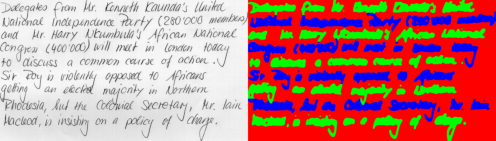
\includegraphics[scale=0.7]{figures/segmentation_eo}
    \caption{Line segmentation by parity}
    \label{FigParityLineSeg}        
\end{figure}

In the following experiments, the input images have been resized to 256x256px and passed to a lightweight U-Net inspired architecture with a Bidirectional LSTM serving as the hidden layer. As opposed to an interesting, but off-topic, model found in literature called U-Net-LSTM used in 3-dimensional image timelapse processing contexts like detection of hydrological topography changes \cite{unetlstm} which has LSTM layers on the skip connections (branches connecting layers of the same shape between the encoder and decoder in order to prevent information loss during down and up sampling \cite{unet}), the model in the current work only replaces the convolution layer "at the bottom of the U" with the recurrent layer, making it more structurally related to the Wave U-Net variant with LSTM applied in 1-D audio signal processing \cite{waveunet}. To the author's awareness, it is the first time such a U-Net with LSTM appended encoder hybrid model is used for text line segmentation in HTR problems. The motivation of the choice for this SegUnetLSTM model resides in the fact it was originally designed for the line segmentation by parity, where a recurrent layer was assigned to take notes on spatial information about the surroundings which is needed in order to label a line as even or odd. The model was eventually left untouched during further experiments. At a later point in this project, the author has also learned about Axler et al.'s heatmap net model which is worth a mention for its capability to reach state of the art results in word level segmentation \cite{wordseg}. The model is used in  Kur{\'e}n et al.'s visual transformer for the HTR \cite{vit_htr}. However, the impressive performance comes at a cost of high computational costs which cross the boundaries proposed for the current work. All the segmentation attempts use some variation of U-Net as their skeleton, one example can be seen in Figure \ref{FigSegArch}.

The model outputs a softmaxed image mask resembling the probabilities of a pixel to be of one of the three categories presented above. At its best run, the model performed great at identifying text areas and filtering out alien objects like drawings, but had a hard time finding a reliable parity line segmentation. The more lines the input contains, the more blurry the output mask becomes. 

\begin{figure}[htbp]
    \centering
        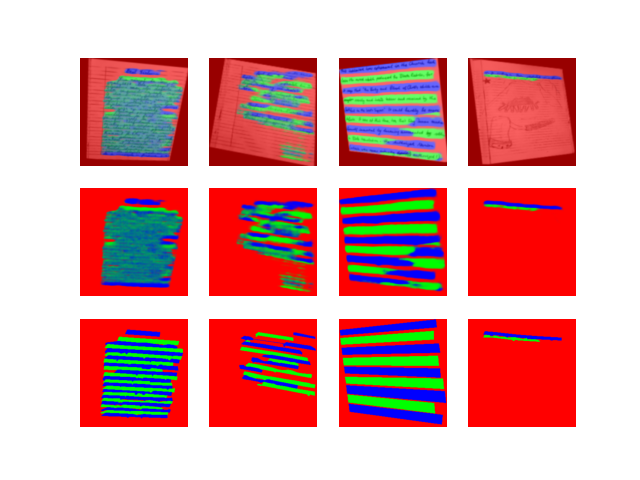
\includegraphics[scale=0.7]{figures/line_seg_parity_result}
    \caption{Line segmentation by parity output. First line: input and overlayed predicted mask. Second line: model output. Third line: ground truth data.}
    \label{FigParityLineSeg}        
\end{figure}

\begin{figure}[htbp]
    \centering
        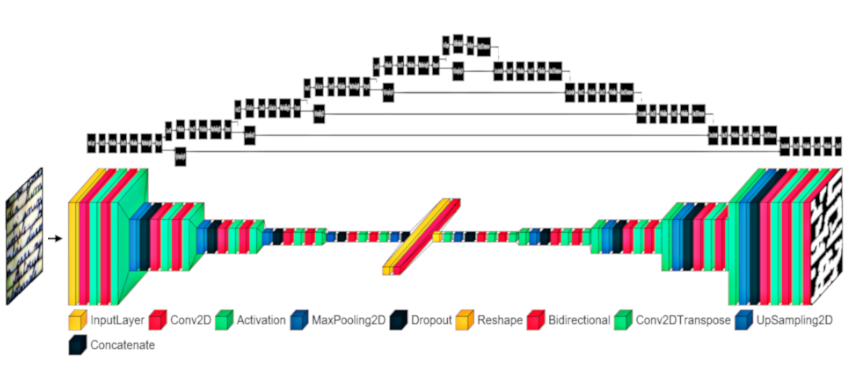
\includegraphics[scale=0.65]{figures/segm_unet.png}
    \caption{Segmentation model architecture (SegUnetLSTM) \cite{visualKeras}}
    \label{FigSegArch}        
\end{figure}

Eventually, the segmentation by parity idea was dropped in favor of a binary mask output. The input image has been split up into 64x64px tiles that are segmented independently (Figure \ref{FixLineSegBin}). The final image is reconstructing by recombining the newly processed tiles into their initial position in the image. It was noted that by including an 8px padding around the tile helps with a more uniform blending at reconstruction time, beside improving the prediction on the edge of the input due to obtaining a broader view of the context. Figure \ref{FigSegPadding} features a segmentation without padding in the left, where it is observed that a text line which crosses two adjacent tiles is split into two upper and lower subsets during segmentation. The addition of padding fixes this issue, while also smoothing the transition in marginal places where predicting the same text line slope from a different tile produces divergent results.

\begin{figure}[htbp]
    \centering
        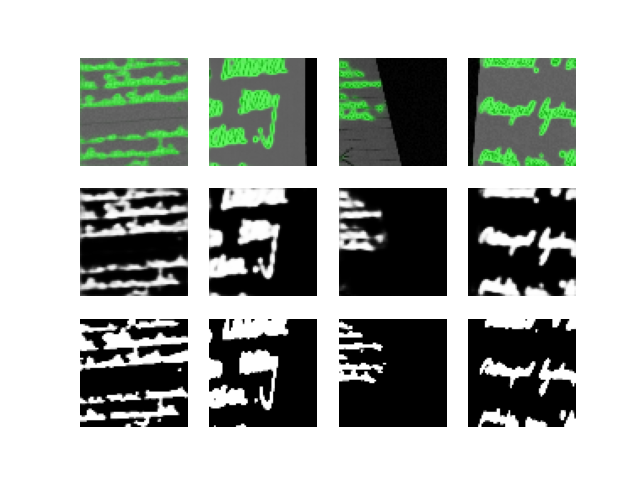
\includegraphics[scale=0.5]{figures/lineseg_bin_64}
    \caption{Text detection in tiles. First line: input and overlayed predicted mask. Second line: model output. Third line: ground truth data.}
    \label{FixLineSegBin}        
\end{figure}

\begin{figure}[htbp]
    \centering
        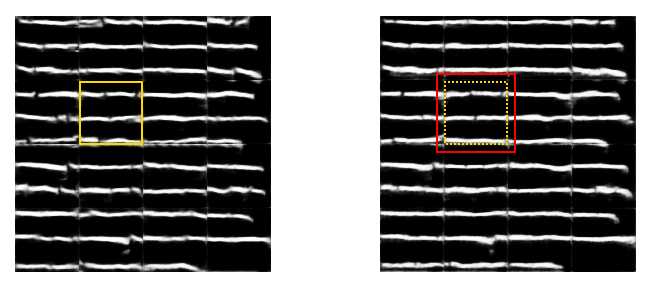
\includegraphics[scale=0.7]{figures/seg_padding.png}
    \caption{The effect of tile padding over the chunkiness aspect of the segmentation}
    \label{FigSegPadding}        
\end{figure}


During the process it was observed that this kind of segmentation is insufficient or difficult to handle in order to achieve line extraction. Therefore, the author has thought of a method to manipulate the previous line parity masks in such a way that minimizes the amount of pixels which are considered text while leaving more blank space between lines. This thinning method starts by identifying connected regions in the output mask using any graph traversal technique. For each region a line is fitted through its pixel coordinates, which is then assigned some stroke proportional to the maximum absolute error, up until a chosen threshold (Figure \ref{FigSegThinning}). Note that this approach may not always end with ideal results, for example, an isolated "t" produces a vertical line. However, we consider this a minor issue that could be corrected in relation with the surrounding context. The main motivation behind the thinning algorithm is that for a longer connected text sequence (which is more likely to encounter in cursive writing), the resulted line offers an approximation for the core area of the text.

\begin{figure}[htbp]
    \centering
        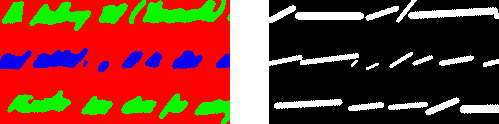
\includegraphics[scale=0.7]{figures/seg_thinning}
    \caption{Thinning.}
    \medskip
    \small
    Left: original hand-made segmentation \\ Right: generated thinned mask    
    \label{FigSegThinning}        
\end{figure}

After a model is trained on the new thinned mask, a postprocessing step follows that rescues the text lines from the segmented data. It is recommended to use the thinned mask (one example in Figure \ref{FigSegSteps} a) to predict the lines count and slopes, and compare them against the normal binary segmented mask (Figure \ref{FigSegSteps} b) to retrieve each lines's individual pixels. A considered heuristic is to make each pixel belong the line whose retraced slope is the closest to.


The line reconstruction or defragmentation is based on the work of Berat et al. \cite{segmChallenging} with slight adjustments to the current context, as shown in the Figure \ref{FigSegFlow}. The reference paper uses ellipse fitting to find the orientation and the trust factor of each connected component. For performance reasons, the current approach considers the direction vector obtained from a linear regression that outputs the standard form of the fitted line equation which prevents numerical instability for vertical lines. The pseudocode describing this process is listed below.

\begin{lstlisting}[language=pascal, escapeinside={[*}{*]}]
function LineFit(x:real*, y:real*)
{ fits a line through points (x_i,y_i) }
{ input: points given by list of real x  and y coordinates }
{ output: real numbers a, b, c, the coefficients of the fitted }
{         line whose equation is expressed as ax+by+c=0 }
  width := max(x)-min(x), height=max(y)-min(y)
  if width>height then
    b0, b1 := LeastSquare(x, y), norm = [*$\sqrt{\mathrm{b0}^2+1}$*]
    a := b0/norm, b:=-1/norm, c:=b1/norm
  else
    b0, b1 := LeastSquare(y, x), norm = [*$\sqrt{\mathrm{b0}^2+1}$*]
    a := -1/norm, b:= b0/norm, c := b1/norm
  end
  (* Normalization step to ensure the direction vector
     always points to the bottom and/or the right *)
  if b<0 or (b=0 and a>0)
    a := -a, b:=-b, c:=-c
  end
  return a,b,c
end
\end{lstlisting}


\begin{figure}[htbp]
    \centering
        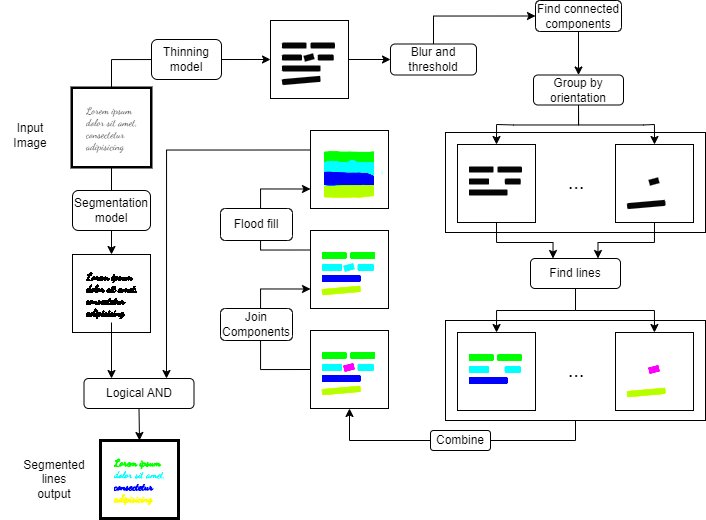
\includegraphics[scale=0.7]{figures/segmentation_flow.png}
    \caption{Segmentation process workflow}
    \label{FigSegFlow}        
\end{figure}

It is crucial to note that this algorithm's output satisfies the relation $a^2+b^2=1$. In other words, The normal vector $(a,b)$ and the direction vector $(b, -a)$ are unit vectors. All the geometrical calculations from now on will include using unit vectors whenever possible since they produce neat and efficient formulae.

Then, we imagine an oriented rectangle around the connected component having two sides parallel with the previously obtained line. The width of the rectangle (length of the sides parallel with the line) is the length of the shortest segment which contains all the points projections on the line, and the height is chosen to be the maximum distance between a point and the fitted line. 

The next step follows with respect to the original work \cite{segmChallenging} by partitioning the mask components which have close orientations into groups. Experimentally, it was considered that a total value of $20$ layers, which gives a rotation sensitivity of $4.5^\circ$, is a sweet spot between performance and reliability. 

\begin{figure}[htbp]
    \centering
        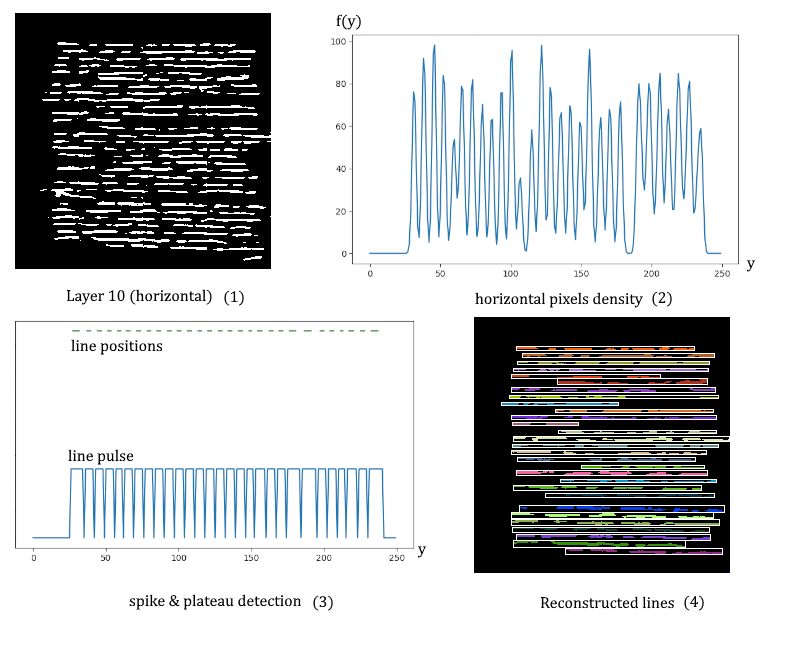
\includegraphics[scale=0.7]{figures/line_reconstruction.png}
    \caption{Line reconstruction example}    
    \label{FigLineRecon}        
\end{figure}

For reuniting lines within the same layer, instead of morphological dilation, a more statistic approach is used to find the potential positions of the lines --- see Figure \ref{FigSegSteps} c,d,e,f. In the first place, the whole binary $mask$ corresponding to each layer is rotated with the angle inverse to its orientation to align the contents to horizontal axis --- Figure \ref{FigLineRecon} (1). Then, we build a cumulative function $f(y)=\sum_{x} mask_{x,y}$
which counts the non-zero pixels on each horizontal line labeled by its coordinate $y$. We expect to have a line in places where the function $f$ reaches its local maxima --- Figure \ref{FigLineRecon} (2). That induces the idea of a simple spike detection in function graph algorithm which retrieves the points $y$ that have a higher value compared to their neighbors. A 1-D convolution may be applied on the cumulative function beforehand to reduce the noisiness of the input, if necessary. As an additional measure, the binary mask can also be preprocessed to remove redundancies, such as performing noise detection with a simple average blur kernel or removing connected components that may have resulted as additional artifacts from the segmentation model (this may occur when text is near an illustration that leads the neural networks into activating chaotically distributed portions of small area on the mask).


\begin{figure}[htbp]
    \centering
        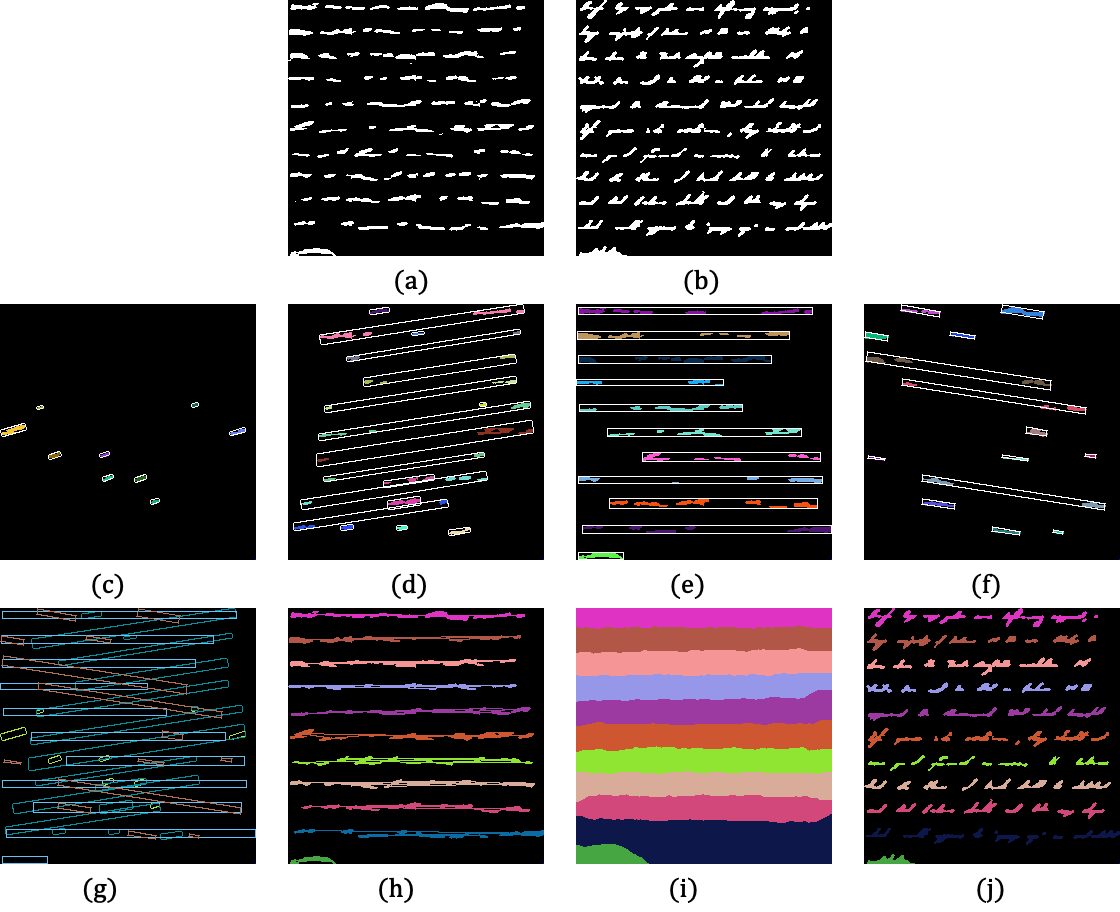
\includegraphics[width=0.7\textwidth]{figures/seg_steps.png}
    \caption{Segmentation steps}
    \label{FigSegSteps}        
\end{figure}

However, knowing about spikes is sometimes not enough to pinpoint lines composed of thick masks (e.g. written with a large font). Thus, the algorithm is complemented by a plateau detection --- see Figure \ref{FigLineRecon} (3). If between two consecutive spikes, or semi-spikes (a point which is a local maximum for one side of its vecinity but not for the other) $y_1<y_2$, the cumulative function satisfies the relation $|f(y)-f(y+1)|<\varepsilon$ foreach $y\in(y_1,y_2)$, where $\varepsilon=10^-2$ is a small chosen tolerance parameter, then the interval $[y_1,y_2]$ spans over a single line. Once the line positions are known, each mask component can be assigned to the line closest to its position --- as shown in Figure \ref{FigLineRecon} (4). 

\begin{figure}[htbp]
    \centering
        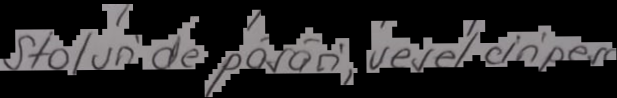
\includegraphics[scale=0.7]{figures/seg_example.png}
    \caption{Example of final segmented line}    
    \label{FigSegmentedLineExample}        
\end{figure}


The process can be improved by further analyzing the properties of all layers and the lines detected within them. For example, some layers may contain misbehaved data (remind the "t" letter whose mask fits to a vertical line despite describing a horizontal text) but in small amounts. Such layers can be dismantled, and their components moved to more trusted lines from other layers, as shown in figure in Figure \ref{FigSegSteps} g, h.

Finally, the segmented lines can be combined with a normal (unthinned --- Figure \ref{FigSegSteps} b) segmented mask in order to complete the line detection. For that, a flood fill algorithm (Figure \ref{FigSegSteps} i) (implemented based on the classical implementation of Lee's algorithm \cite{lee} customized to work with multiple starting contour points) starting from each line mask simultaneously is applied to create a full partition of the mask's canvas only in terms of line labels. This heat map tells each pixels what line it belongs to, which is sufficient to provide a clear delimitation of lines in the normal mask by simply performing an elementwise logical and operation between the two images --- Figure \ref{FigSegSteps} j. Last but not least, each line can be cut from the original input image according to the segmentation (see Figure \ref{FigSegmentedLineExample}) and further passed to the recognition model.